\documentclass[tikz]{standalone}
\usepackage{pgfplots}
\pgfplotsset{compat=1.15}
\usepackage{mathrsfs}
\usetikzlibrary{arrows,calc}
\usepackage{tkz-euclide}
\pagestyle{empty}

\definecolor{AngleClr}{rgb}{0,0.39215686274509803,0}
\definecolor{ShapeClr}{rgb}{0.6,0.2,0}
\definecolor{SquareClr}{RGB}{250, 248, 217}


\begin{document}

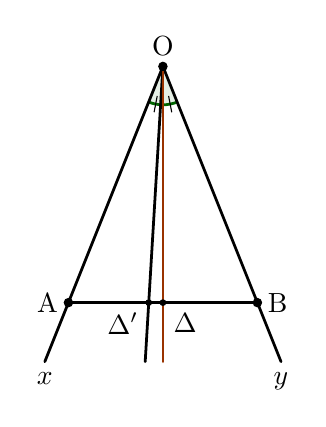
\begin{tikzpicture}[scale=.75]
\tkzSetUpLine[line width=1pt,color=black]
\tkzSetUpPoint[fill=black]

\tkzDefPoints{0/0/x,2/5/O,4/0/y,2/0/d,2/1/S,1.7/0/DDD,4/1/XX}

\tkzInterLL(S,XX)(O,x) \tkzGetPoint{A}
\tkzInterLL(S,XX)(O,y) \tkzGetPoint{B}
\tkzInterLL(S,XX)(O,DDD) \tkzGetPoint{DD}

\tkzFillAngles[fill=AngleClr,size=.65,fill opacity=0.1](A,O,S S,O,B)
\tkzMarkAngles[line width=1pt,size=.65,color=AngleClr,mark=|,mksize=3](A,O,S S,O,B)

\tkzDrawSegments[line width=1pt,color=black](x,O y,O)
\tkzDrawSegments[line width=1pt,color=black](A,B O,DDD)
\tkzDrawSegment[line width=1pt,color=ShapeClr](d,O)


\tkzDrawPoints[size=3](O,A,B)
\tkzDrawPoints[size=2](DD,S)


\tkzLabelPoint[below](x){$x$}
\tkzLabelPoint[below](y){$y$}
\tkzLabelPoint[left](A){$\rm A$}
\tkzLabelPoint[right](B){$\rm B$}
\tkzLabelPoint[below right](S){$\rm \Delta$}
\tkzLabelPoint[below left](DD){$\rm \Delta'$}

\tkzLabelPoint[above](O){$\mathrm{O}$}

\end{tikzpicture}

\end{document}
